\documentclass [tikz] {standalone}

%common figure styles
\input{header.htex}


\begin {document}
%\begin{figure}[ht!]
%	\begin{center}
		
		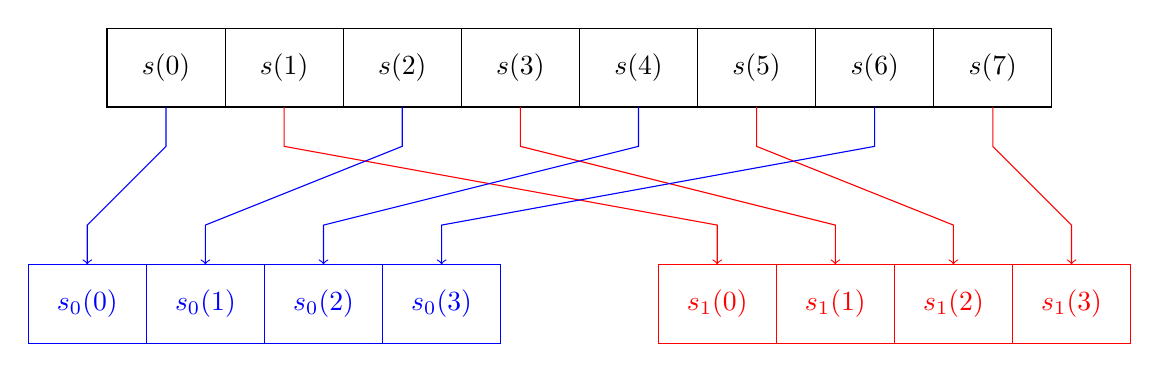
\begin{tikzpicture}
		
			\foreach \z in {0, 1, ...,7}
			{
				\draw	(\z*1.5 +1, 0) rectangle (\z*1.5+2.5, -1);
				
				\draw(\z*1.5 + 1.75, -0.5) node {$s(\z)$};		
			}
			
			\foreach \z in {0, 1, 2, 3}
			{
				\draw[blue]	(\z*1.5, -3) rectangle (\z*1.5+1.5, -4);
				\draw[blue] (\z*1.5 + 0.75, -3.5) node {$s_0(\z)$};
				
				\draw[->, blue] (\z*3 + 1.75, -1) -- (\z*3 + 1.75, -1.5) -- (\z*1.5 + 0.75, -2.5) -- (\z*1.5 + 0.75, -3);
				
				
				
				\draw[red]	(\z*1.5 + 8, -3) rectangle (\z*1.5+9.5, -4);
				\draw[red] (\z*1.5 + 8.75, -3.5) node {$s_1(\z)$};
				
					\draw[->, red] (\z*3 + 3.25, -1) -- (\z*3 + 3.25, -1.5) -- (\z*1.5 + 8.75, -2.5) -- (\z*1.5 + 8.75, -3);
					
						
			}
			
			
			
		
		\end{tikzpicture}
\end {document}

		
%		\caption{Прореживание по времени для $N=8$ }\label{fft_dec_in_time:fig1}
%	\end{center}
%\end{figure}